\documentclass[12pt,a4paper]{article}

%\usepackage[left=1.5cm,right=1.5cm,top=1cm,bottom=2cm]{geometry}
\usepackage[in, plain]{fullpage}
\usepackage{array}
\usepackage{../../../pas-math}
\usepackage{../../../moncours}
\usepackage{textcomp}


%\usepackage{pas-cours}
%-------------------------------------------------------------------------------
%          -Packages nécessaires pour écrire en Français et en UTF8-
%-------------------------------------------------------------------------------
\usepackage[utf8]{inputenc}
\usepackage[frenchb]{babel}
\usepackage[T1]{fontenc}
\usepackage{lmodern}
\usepackage{textcomp}



%-------------------------------------------------------------------------------

%-------------------------------------------------------------------------------
%                          -Outils de mise en forme-
%-------------------------------------------------------------------------------
\usepackage{hyperref}
\hypersetup{pdfstartview=XYZ}
%\usepackage{enumerate}
\usepackage{graphicx}
\usepackage{multicol}
\usepackage{tabularx}
\usepackage{multirow}


\usepackage{anysize} %%pour pouvoir mettre les marges qu'on veut
%\marginsize{2.5cm}{2.5cm}{2.5cm}{2.5cm}

\usepackage{indentfirst} %%pour que les premier paragraphes soient aussi indentés
\usepackage{verbatim}
\usepackage{enumitem}
\usepackage[usenames,dvipsnames,svgnames,table]{xcolor}

\usepackage{variations}

%-------------------------------------------------------------------------------


%-------------------------------------------------------------------------------
%                  -Nécessaires pour écrire des mathématiques-
%-------------------------------------------------------------------------------
\usepackage{amsfonts}
\usepackage{amssymb}
\usepackage{amsmath}
\usepackage{amsthm}
\usepackage{tikz}
\usepackage{xlop}
%-------------------------------------------------------------------------------



%-------------------------------------------------------------------------------


%-------------------------------------------------------------------------------
%                    - Mise en forme avancée
%-------------------------------------------------------------------------------

\usepackage{ifthen}
\usepackage{ifmtarg}


\newcommand{\ifTrue}[2]{\ifthenelse{\equal{#1}{true}}{#2}{$\qquad \qquad$}}

%-------------------------------------------------------------------------------

%-------------------------------------------------------------------------------
%                     -Mise en forme d'exercices-
%-------------------------------------------------------------------------------
%\newtheoremstyle{exostyle}
%{\topsep}% espace avant
%{\topsep}% espace apres
%{}% Police utilisee par le style de thm
%{}% Indentation (vide = aucune, \parindent = indentation paragraphe)
%{\bfseries}% Police du titre de thm
%{.}% Signe de ponctuation apres le titre du thm
%{ }% Espace apres le titre du thm (\newline = linebreak)
%{\thmname{#1}\thmnumber{ #2}\thmnote{. \normalfont{\textit{#3}}}}% composants du titre du thm : \thmname = nom du thm, \thmnumber = numéro du thm, \thmnote = sous-titre du thm

%\theoremstyle{exostyle}
%\newtheorem{exercice}{Exercice}
%
%\newenvironment{questions}{
%\begin{enumerate}[\hspace{12pt}\bfseries\itshape a.]}{\end{enumerate}
%} %mettre un 1 à la place du a si on veut des numéros au lieu de lettres pour les questions 
%-------------------------------------------------------------------------------

%-------------------------------------------------------------------------------
%                    - Mise en forme de tableaux -
%-------------------------------------------------------------------------------

\renewcommand{\arraystretch}{1.7}

\setlength{\tabcolsep}{1.2cm}

%-------------------------------------------------------------------------------



%-------------------------------------------------------------------------------
%                    - Racourcis d'écriture -
%-------------------------------------------------------------------------------

% Angles orientés (couples de vecteurs)
\newcommand{\aopp}[2]{(\vec{#1}, \vec{#2})} %Les deuc vecteurs sont positifs
\newcommand{\aopn}[2]{(\vec{#1}, -\vec{#2})} %Le second vecteur est négatif
\newcommand{\aonp}[2]{(-\vec{#1}, \vec{#2})} %Le premier vecteur est négatif
\newcommand{\aonn}[2]{(-\vec{#1}, -\vec{#2})} %Les deux vecteurs sont négatifs

%Ensembles mathématiques
\newcommand{\naturels}{\mathbb{N}} %Nombres naturels
\newcommand{\relatifs}{\mathbb{Z}} %Nombres relatifs
\newcommand{\rationnels}{\mathbb{Q}} %Nombres rationnels
\newcommand{\reels}{\mathbb{R}} %Nombres réels
\newcommand{\complexes}{\mathbb{C}} %Nombres complexes


%Intégration des parenthèses aux cosinus
\newcommand{\cosP}[1]{\cos\left(#1\right)}
\newcommand{\sinP}[1]{\sin\left(#1\right)}


%Probas stats
\newcommand{\stat}{statistique}
\newcommand{\stats}{statistiques}
%-------------------------------------------------------------------------------

%-------------------------------------------------------------------------------
%                    - Mise en page -
%-------------------------------------------------------------------------------

\newcommand{\twoCol}[1]{\begin{multicols}{2}#1\end{multicols}}


\setenumerate[1]{font=\bfseries,label=\textit{\alph*})}
\setenumerate[2]{font=\bfseries,label=\arabic*)}


%-------------------------------------------------------------------------------
%                    - Elements cours -
%-------------------------------------------------------------------------------





%\makeatletter
%\renewcommand*{\@seccntformat}[1]{\csname the#1\endcsname\hspace{0.1cm}}
%\makeatother


%\author{Olivier FINOT}
\date{}
\title{Se repérer dans l'espace}

%\newcommand{\disp}{false}

%\lhead{CH1 : Calculs numériques}
%\rhead{O. FINOT}
%
%\rfoot{Page \thepage}
\begin{document}
	\maketitle
	
	%\chap[num=1, color=red]{Se repérer dans l'espace}{Olivier FINOT, \today }
	
	\begin{myobj}
	\begin{itemize}
		
		\item Construire le symétrique d’un point ou d'une figure par rapport à une droite à la main où à l’aide d’un logiciel;
		\item Construire le symétrique d’un point ou d'une figure par rapport à un point, à la main où à l’aide d’un logiciel;
		\item Utiliser les propriétés de la symétrie axiale ou centrale;
		\item Identifier des symétries dans des figures.		
	\end{itemize}
\end{myobj}

\begin{mycomp}
	\begin{itemize}
		\item \kw{Chercher (Ch2)} :  s’engager    dans    une    démarche    scientifique, observer, questionner, manipuler, expérimenter (sur une feuille de papier, avec des objets, à l’aide de logiciels), émettre des hypothèses, chercher des exemples ou des contre-exemples, simplifier ou particulariser une situation, émettre une conjecture ;
		\item \kw{Raisonner (Ra3)} :  démontrer : utiliser un raisonnement logique et des règles établies (propriétés, théorèmes, formules) pour parvenir à une conclusion ;
		\item \kw{Communiquer (Co2)} :  expliquer à l’oral ou à l’écrit (sa démarche, son raisonnement, un calcul, un protocole   de   construction   géométrique, un algorithme), comprendre les explications d’un autre et argumenter dans l’échange ; 
		
	\end{itemize}
\end{mycomp}




\section{Repérage dans un parallélépipède rectangle}

\begin{myact}
	Activité 1 page 161
\end{myact}


\begin{mydef}

	Dans un parallélépipède rectangle, un \textbf{repère} est formé par trois arêtes ayant un sommet commun appelé \textbf{origine du repère}.

\end{mydef}

\begin{myprop}
	Tout point d'un parallélépipède rectangle est repéré par trois nombre, ses \textbf{coordonnées} : l'\textcolor{red}{abscisse}, l'\textcolor{green}{ordonnée}, l'\textcolor{blue}{altitude}.
\end{myprop}

\begin{myex}
	
	\begin{multicols}{2}
	ABCDEFGH est un parallélépipède rectangle. 
	Le repère formé par les arêtes $[AB]$, $[AD]$ et $[AE]$ a pour origine le point A. On le note (\textbf{A;B,D,E}).
	
	Les coordonnées du point D sont \mycoord{0}{1}{0}.\\
	
	De même, A\mycoord{0}{0}{0}, B\mycoord{1}{0}{0}, E\mycoord{0}{0}{1}.\\
	
	Le point M est "à la verticale" de C : il a même abscisse et même ordonnées que C, mais comme il se situe au milieu l'arête $[CG]$, son altitude est \num{0.5}. 
	
	Ainsi M\mycoord{1}{1}{0.5}
%	\vspace*{1cm} 
	%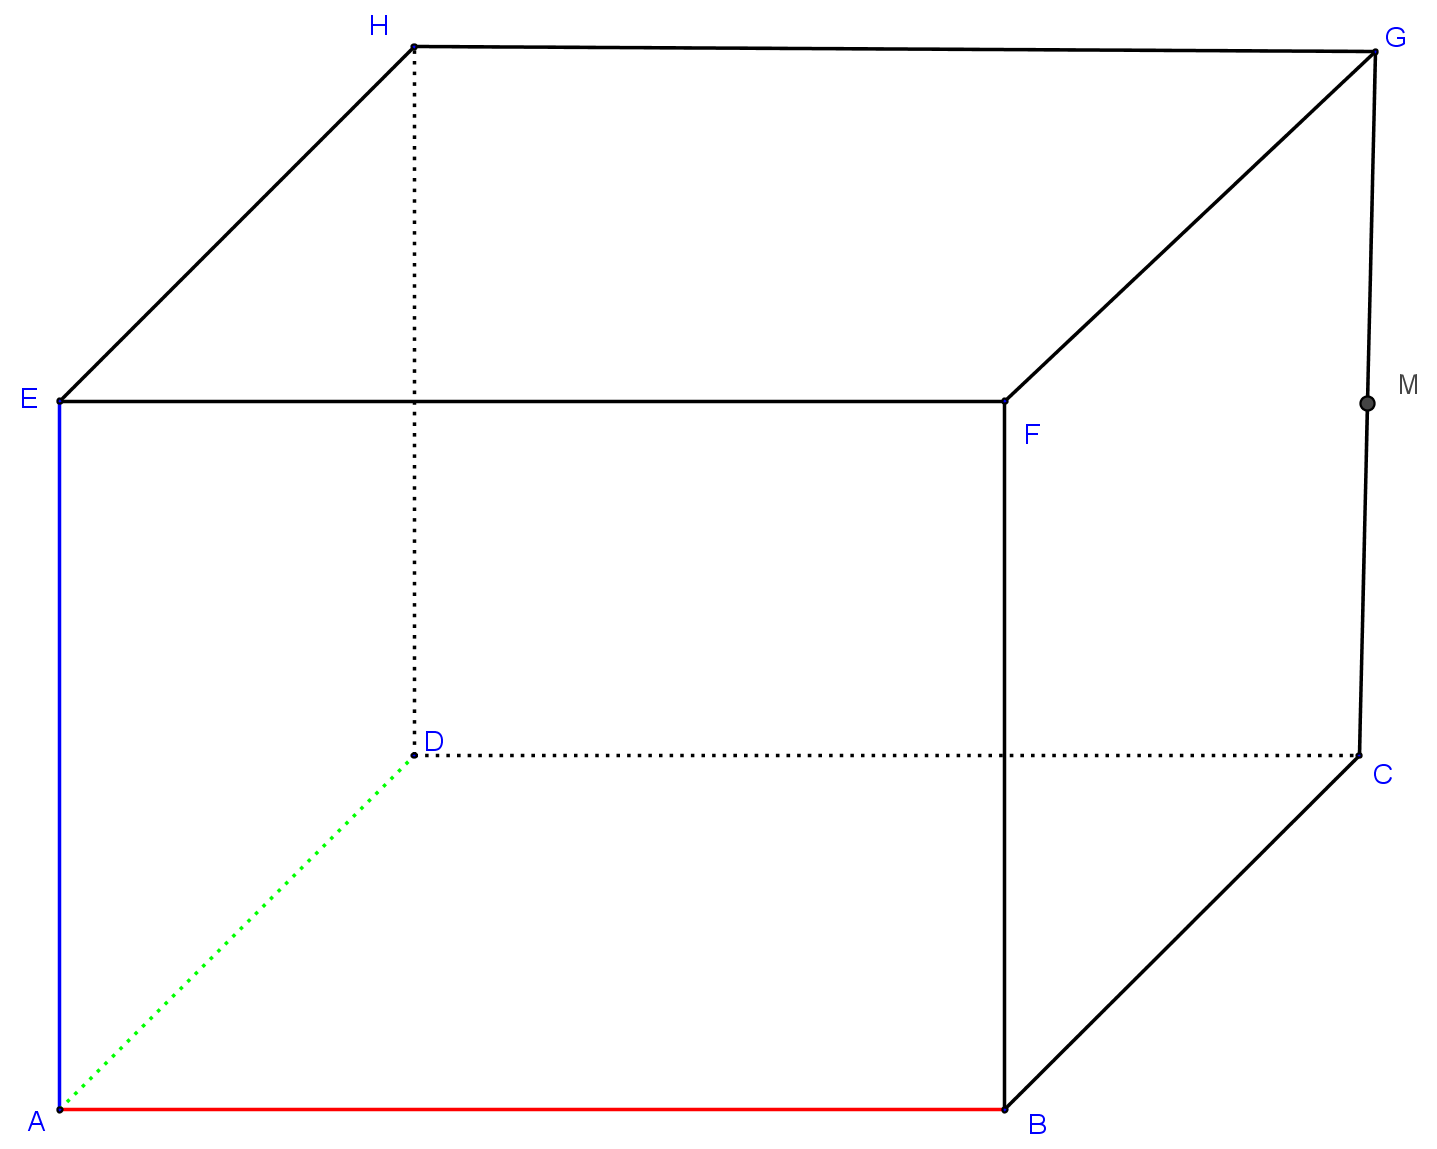
\includegraphics[scale=0.22]{figure}
	\begin{center}
		
	\definecolor{uuuuuu}{rgb}{0.26666666666666666,0.26666666666666666,0.26666666666666666}
	\definecolor{qqffqq}{rgb}{0.,1.,0.}
	\definecolor{ffqqqq}{rgb}{1.,0.,0.}
	\definecolor{qqqqff}{rgb}{0.,0.,1.}
	\begin{tikzpicture}[scale=0.55, line cap=round,line join=round,>=triangle 45,x=1.0cm,y=1.0cm]
	\clip(-4.36,-1.26) rectangle (18.64,9.88);
	\draw [line width=1.2pt,color=ffqqqq] (-1.,0.)-- (7.,0.);
	\draw [line width=1.2pt] (7.,6.)-- (7.,0.);
	\draw [line width=1.2pt] (7.,6.)-- (-1.,6.);
	\draw [line width=1.2pt,color=qqqqff] (-1.,6.)-- (-1.,0.);
	\draw [line width=1.2pt] (7.,0.)-- (10.,3.);
	\draw [line width=1.2pt] (10.,3.)-- (10.14,8.96);
	\draw [line width=1.2pt] (7.,6.)-- (10.14,8.96);
	\draw [line width=1.2pt] (-1.,6.)-- (2.,9.);
	\draw [line width=1.2pt] (2.,9.)-- (10.14,8.96);
	\draw [line width=1.2pt,dotted,color=qqffqq] (-1.,0.)-- (2.,3.);
	\draw [line width=1.2pt,dotted] (2.,3.)-- (10.,3.);
	\draw [line width=1.2pt,dotted] (2.,3.)-- (2.,9.);
	\begin{scriptsize}
	\draw [fill=qqqqff] (-1.,0.) circle (0.5pt);
	\draw[color=qqqqff] (-1.22,-0.02) node {$A$};
	\draw [fill=qqqqff] (7.,0.) circle (0.5pt);
	\draw[color=qqqqff] (7.26,-0.04) node {$B$};
	\draw [fill=qqqqff] (-1.,6.) circle (0.5pt);
	\draw[color=qqqqff] (-1.28,6.1) node {$E$};
	\draw [fill=qqqqff] (7.,6.) circle (0.5pt);
	\draw[color=qqqqff] (7.22,5.8) node {$F$};
	\draw [fill=qqqqff] (10.,3.) circle (0.5pt);
	\draw[color=qqqqff] (10.18,2.92) node {$C$};
	\draw [fill=qqqqff] (10.14,8.96) circle (0.5pt);
	\draw[color=qqqqff] (10.28,9.16) node {$G$};
	\draw [fill=qqqqff] (2.,9.) circle (0.5pt);
	\draw[color=qqqqff] (1.68,9.26) node {$H$};
	\draw [fill=qqqqff] (2.,3.) circle (0.5pt);
	\draw[color=qqqqff] (2.14,3.2) node {$D$};
	\draw [fill=uuuuuu] (10.07,5.98) circle (1.5pt);
	\draw[color=uuuuuu] (10.38,6.22) node {$M$};
	\end{scriptsize}
	\end{tikzpicture}

	\end{center} 
	\end{multicols}
\end{myex}

\section{Repérage sur la Terre}

\begin{myact}{B}
	Activité 2 p 161
	
	Les coordonnées géographiques de Oran sont $0$° Est et $35$° Nord.
	
	Celles de Kerguelen sont $70$° Est et $50$° Sud.
	
	Celles de Galapagos sont $90$° Ouest et $0$° Nord.
\end{myact}


\begin{mydef}
	On considère que la Terre est une sphère.
	
	L'origine du repère est le centre de la Terre, les axes sont 
	\begin{itemize}
		\item Un cercle : l'\kw{équateur};
		\item Un demi-cercle : le \kw{méridien de Greenwich}.
	\end{itemize}
	
	La Terre est quadrillée par des cercles \kw{parallèles} à l'équateur, et des demi-cercles allant d'un pôle à l'autre, appelés \kw{méridiens} :
	
	\begin{multicols}{2}
				\begin{itemize}
			\item L'abscisse d'un point correspond à l'angle, orienté Ouest ou Est, entre le méridien de Greenwich et le méridien du point. C'est sa \kw{longitude}.
			\item L'ordonnée d'un point correspond à l'angle, orienté Nord ou Sud, entre l'équateur et le parallèle du point. C'est sa \kw{latitude}.
		\end{itemize}
		
		\begin{center}
			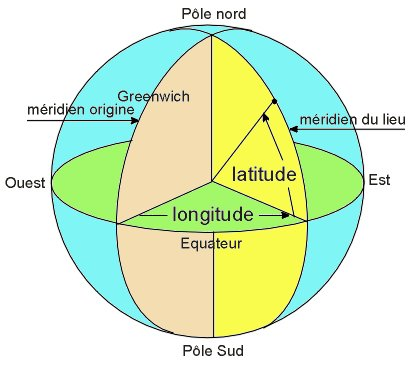
\includegraphics[scale=0.55]{img/terre}
		\end{center}
		
	\end{multicols}
	
\end{mydef}

\begin{myex}
	\begin{multicols}{2}
		\begin{center}
			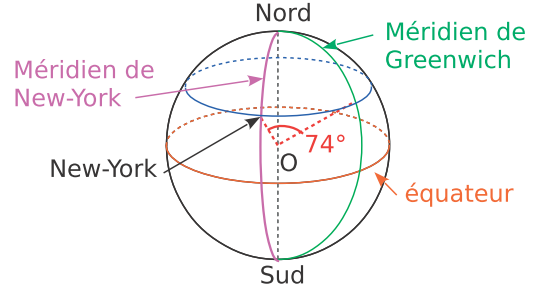
\includegraphics[scale=0.5]{img/terre1}
		\end{center}
		La longitude de New York est $74$° Ouest.
		
		\begin{center}
			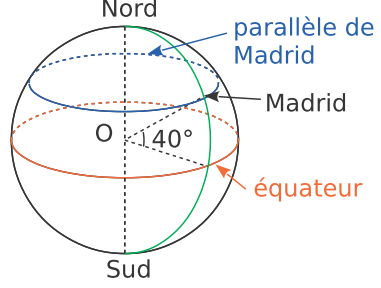
\includegraphics[scale=0.5]{img/terre2}
		\end{center}
		La latitude de Madrid est $40$° Nord.
	\end{multicols}
\end{myex}
\end{document}